\chapter{Interface de Usuário}
\label{c:interface_de_usuario}
% ---
Todo o sistema para alimentação dos dados de consumo, bem como a estrutura dos dados em si está definida, porém falta um sistema capaz se possibilitar uma visualização real pelo usuário dos dados coletas, bem como uma interface que permita que sejam cadastrados dados de gerenciamento dos dispositivos de medição.

Para isso foi desenvolvida a interface \textit{web} do SIDE, como sendo a interface principal do sistema, sendo ela a responsável por cadastro de usuários para a utilização do sistema, visualização dos dados de medição dos medidores CCK, cadastro das unidades consumidoras, visualização georreferenciada dos dispositivos instalados, entre outras.

\section{Uso do \textit{CUBA Framework}}

Para o desenvolvimento da Interface do SIDE, foi escolhida a linguagem de programação Java com o uso de um \textit{framework} que possibilitasse o desenvolvimento ágil facilitando na criação das entidades e seus respectivos relacionamentos e desse base para a criação de uma boa visualização para o usuário. 

A plataforma escolhida para desenvolvimento foi o \textit{CUBA Framework}, utilizado em sua versão 6.10 cuja a documentação pode ser acessada através do anexo \ref{anex:doc-cuba}.

A interface de usuário disponibilizada pelo CUBA pode ser tanto uma interface padrão utilizando \textit{Spring} quando uma interface mais personalizável utilizando \textit{Polymer 2}, que é um framework JavaScript da empresa Google para desenvolvimento web baseado na utilização de \textit{Web Components}, que foi a escolhida para o desenvolvimento deste projeto.

\section{Uso da biblioteca \textit{Polymer 2}}

Escolhida a Interface de uso Polymer precisa-se entender melhor os padrões de desenvolvimento que a mesma utiliza.

O Polymer é uma biblioteca JavaScript usada para a criação de aplicações web usando o conceito de \textit{Web Components}. Esses \textit{Web Components} podem ser descritos como elementos reutilizáveis que podem ser inseridos em páginas ou aplicações \textit{web}, podendo inclusive ser mesclado com outras bibliotecas JavaScript. O Polymer é como um bloco de montar, que pode ser encaixado de diversas maneiras para construir diferentes tipos de aplicações. 

Nesta versão do CUBA é utilizada a versão 2 do Polymer, cuja a documentação pode ser acessada através do anexo \ref{anex:doc-polymer}.

\section{Telas do SIDE}

Descrito os frameworks utilizados, pode-se agora definir os modos de funcionamento das telas desenvolvidas para o sistema. 

\subsection{Login}

A tela inicial do sistema é a tela de login, responsável pela autenticação do usuário cadastrado no sistema, gerando uma chave de sessão válida para o mesmo, liberando assim o seu acesso ao sistema.

Esta tela permite também a troca da senha atual do usuário, enviando uma nova senha temporária para o endereço de e-mail cadastrado para o mesmo. Abaixo temos uma imagem da tela de login:

\begin{figure}[H]
    \centering
    \caption{Tela de Login do SIDE}
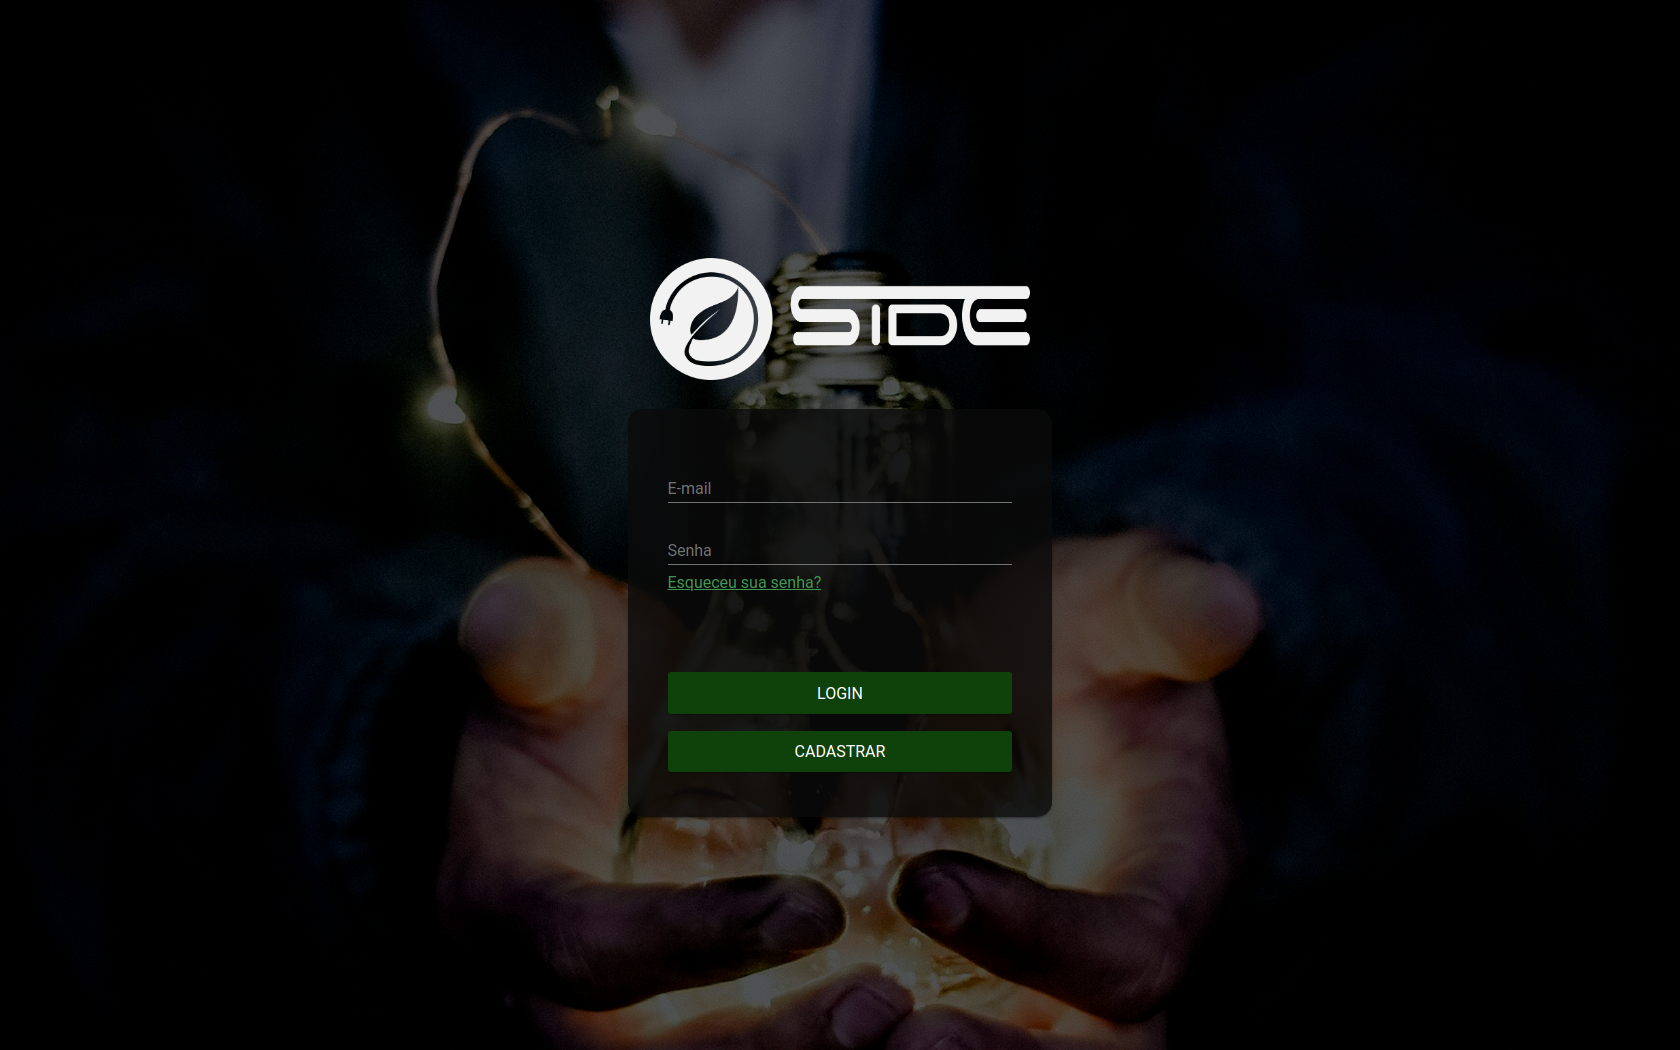
\includegraphics[width=\linewidth]{imagens/side/side-login.png}
    \caption*{Fonte: Próprio Autor}
    \label{fig:side-login}
\end{figure}


Além disso caso não possua acesso ainda, pode ser feito o cadastro do usuário, fornecendo seu nome, e-mail, cpf, e a senha desejada. Este cadastro irá gerar um acesso básico ao sistema que poderá ser controlado pelo administrador do sistema. Abaixo temos uma imagem da tela de cadastro:

\begin{figure}[H]
    \centering
    \caption{Tela de Cadastro do SIDE}
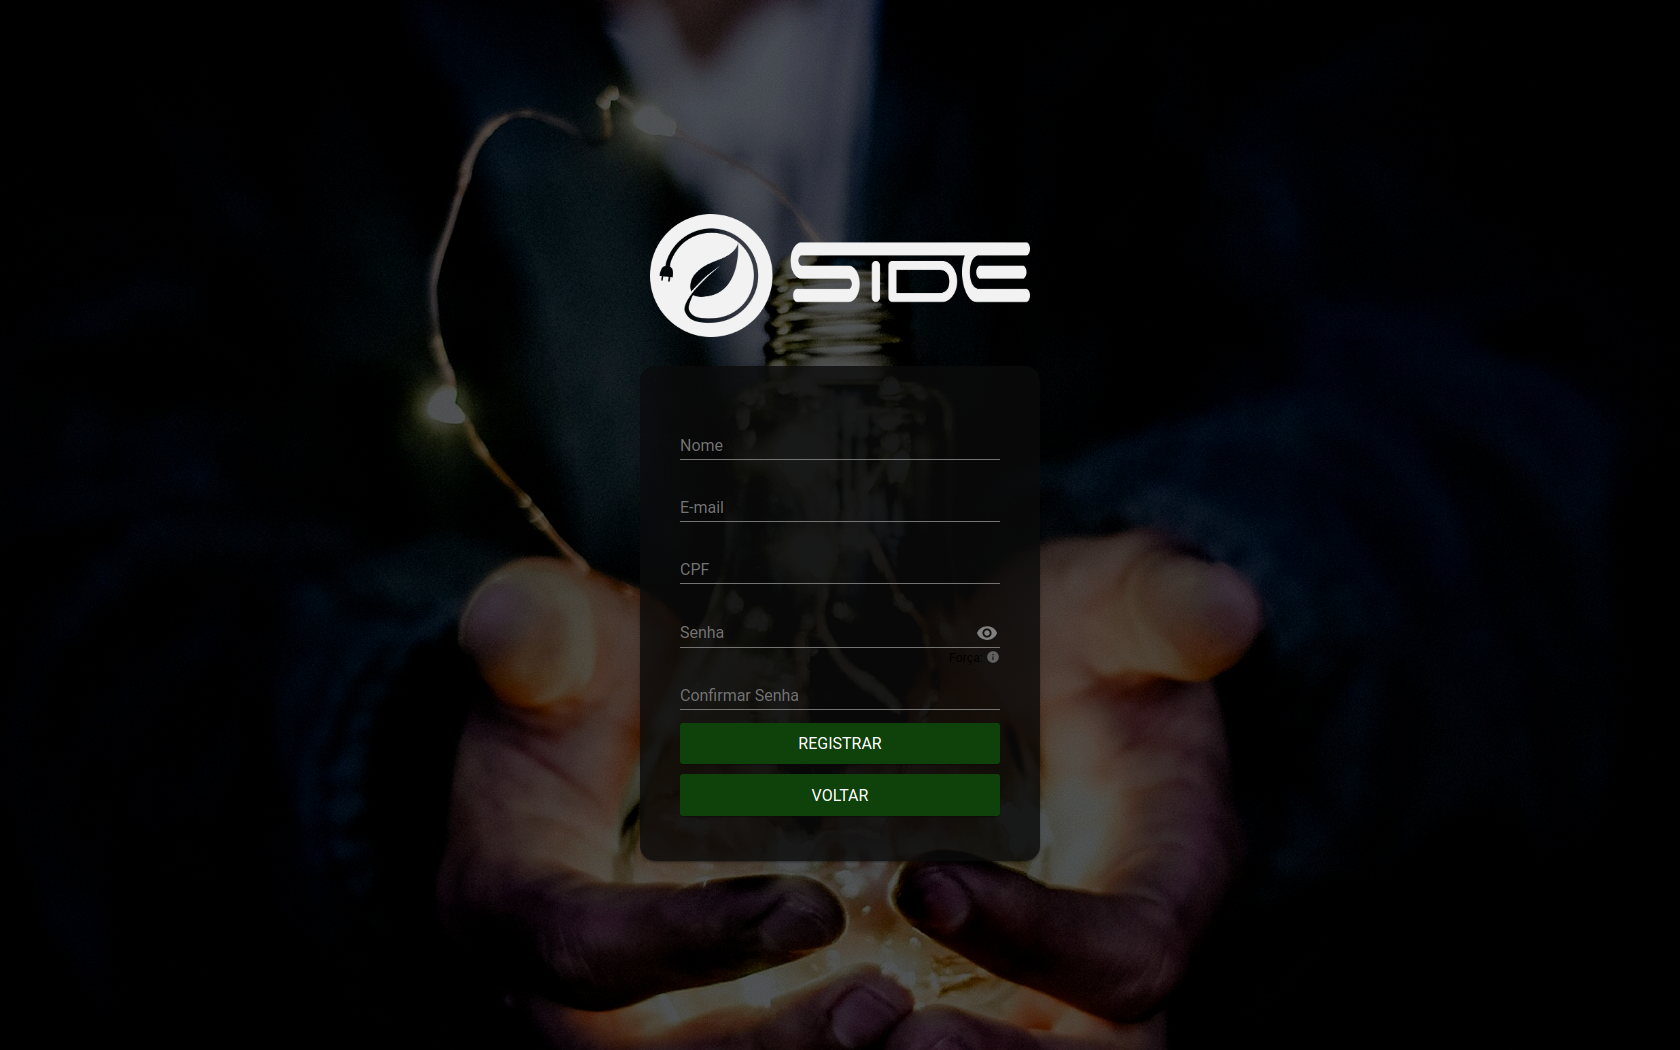
\includegraphics[width=0.7\linewidth]{imagens/side/side-cadastro.png}
    \caption*{Fonte: Próprio Autor}
    \label{fig:side-cadastro}
\end{figure}

\subsection{Tela Principal}

Após autenticado no sistema o usuário tem acesso ao uso do SIDE, onde inicialmente ele verá um mapa com todos os pontos de medição cadastrado no sistema que possuam suas coordenadas geográficas cadastradas. Esses pontos podem ser clicados, fornecendo informações mais detalhadas como consumo atual através da última leitura, denominação, data da última leitura, unidade consumidora vinculada à ele, e o tipo de medidor.

O mapa foi construído em cima de um \textit{Web Component} do Polymer fornecido pela Google para acesso a api do Google Maps. Abaixo temos uma imagem da \textit{home} do sistema.

\begin{figure}[H]
    \centering
    \caption{Tela Principal do SIDE}
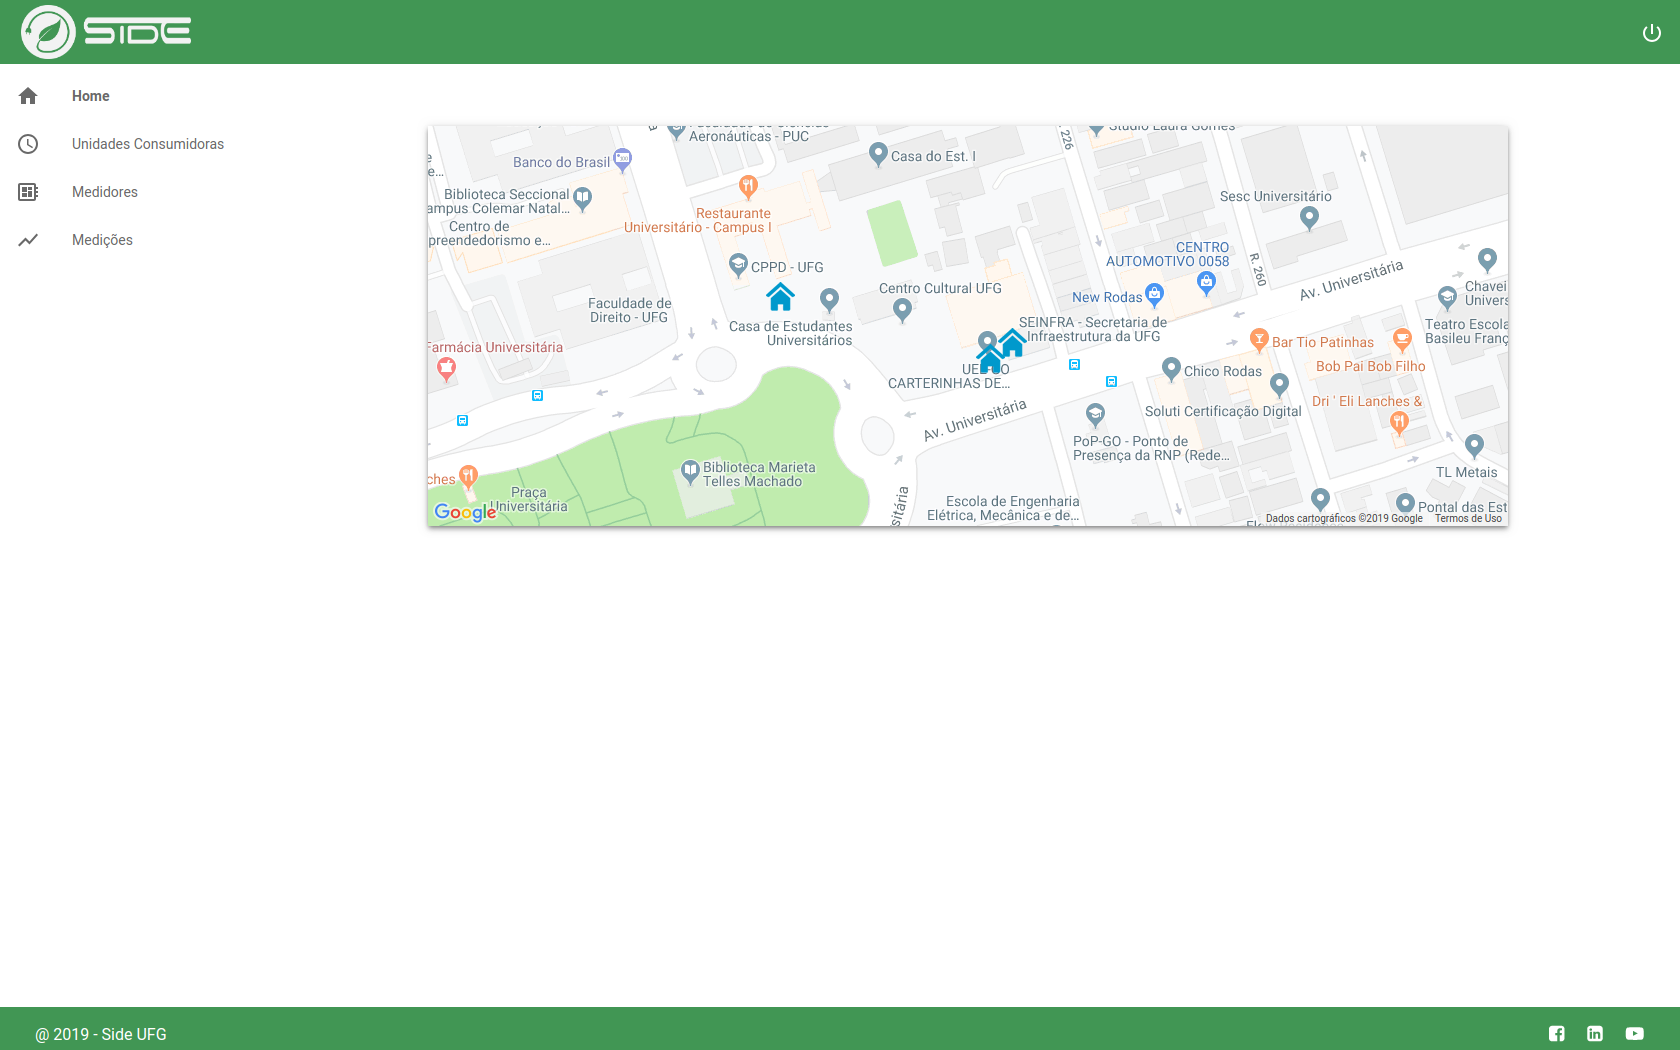
\includegraphics[width=0.7\linewidth]{imagens/side/side-home.png}
    \caption*{Fonte: Próprio Autor}
    \label{fig:side-home}
\end{figure}


\subsection{Cadastro de Medidores}

\subsection{Cadastro de Unidades Consumidoras}

\subsection{Visualização de Medições}